%%%%%%%%%%%%%%%%%%%%%%%%%%%%%%%%%%%%%%%%%%%%%%
\documentclass[11pt,a4paper]{article} %define the document class
\usepackage[latin1]{inputenc} %encode related

%using equations, math fonts
\usepackage{amsmath,bm,amsthm,amssymb}

%using contents tables, index
\usepackage{makeidx}

%using graphs
\usepackage{graphicx}

%for locating tables. graphs
\usepackage{float}

%using colors, links
\usepackage{color}
\usepackage{xcolor}
\usepackage[colorlinks,linkcolor=blue,anchorcolor=blue,citecolor=blue]{hyperref}

%%% For XeTeX
%\usepackage{fontspec}
%\setsansfont{DejaVu Serif}%
%\setmainfont[Mapping=tex-text]{Times New Roman} %

%data time related
\usepackage[level]{datetime}

%Citation style
\usepackage[authoryear]{natbib} %for author year style
%\usepackage{natbib} %normal style


%all kinds of marks, signs
\usepackage{wasysym}
\usepackage{marvosym}

%If you want to specify the content size on the page
\usepackage{geometry}
\geometry{left=2.5cm,right=2.5cm,top=2.5cm,bottom=2.5cm}

%if you want to count pages 
\usepackage{lastpage}

%Page heads and foots
\usepackage{fancyhdr}
\pagestyle{fancy}
\fancyhf{}
\fancyhead[L]{\scriptsize\textit{Left Page Head}}
\fancyhead[R]{\scriptsize\textit{\color{green}{Right Page Head}}}
\fancyfoot[R]{\scriptsize{page \thepage/\pageref{LastPage}}}
\fancyfoot[L]{\scriptsize\textit{Left Page Foot	}}
\renewcommand{\headrulewidth}{0pt} %hide the line
\setlength{\headsep}{0.5cm} %set the separation

%support author block
\usepackage{authblk}

%%%%%%%%%%%%%%%%%%%%%%%%%%%%%%%%%%%%%%%%%%%%%%
%%%%%%%%%%%%%%%%%%%%%%%%%%%%%%%%%%%%%%%%%%%%%%
%%%%%%%%%%%%%%%%%%  TITLE and AUTHORS %%%%%%%%%
%%%%%%%%%%%%%%%%%%%%%%%%%%%%%%%%%%%%%%%%%%%%%%
%%%%%%%%%%%%%%%%%%%%%%%%%%%%%%%%%%%%%%%%%%%%%%
%Title and author
\title{This is the title of an Article}
\author[1]{ {\TeX}pen\thanks{\href{http://www.journalhome.com/texpen/}{http://www.journalhome.com/texpen/}}}
\author[2]{MengChang Wang\thanks{wangmc@ntu.edu.sg}}
\affil[1]{{\small \textit{http://www.journalhome.com/texpen/}}}
\affil[2]{{\small \textit{Nanyang Technological University, Singapore}}}
%%%%%%%%%%%%%%%%%%%%%%%%%%%%%%%%%%%%%%%%%%%%%%

%%%%% PDF Propertity Info
\hypersetup{pdfauthor={Author},%
            pdftitle={A document prepared with TeXpen},%
            pdfsubject={the subject},%
            pdfkeywords={one, two},%
            pdfproducer={LaTeX},%
            pdfcreator={LaTeX and TeXpen}
}

%%% Drawing a picture
%\usepackage[Gray]{SIunits}
%\usepackage{colortbl}
%\usepackage[dvipsnames,pdftex,fixpdftex]{xcolor}
\usepackage{tikz}
\usetikzlibrary{decorations.pathmorphing}

\begin{document}

%%%%%%%%%%%%%%%%%%%%%%%%%%%%%%%%%%%%%%%%%%%%%%
%%%%%%%%%%%%%%%%%%%%%%%%%%%%%%%%%%%%%%%%%%%%%%
%%%%%%%%%%%%%%%%%%%%%%%%%%%%%%%%%%%%%%%%%%%%%%
%%%               Your Content Here
%%%%%%%%%%%%%%%%%%%%%%%%%%%%%%%%%%%%%%%%%%%%%%
%%%%%%%%%%%%%%%%%%%%%%%%%%%%%%%%%%%%%%%%%%%%%%

%%make the title and author list and footnotes
\maketitle

%%%%%%%  ABSTRACT HERE %%%%%%
\begin{abstract}
This paper is to demonstrate that you have done well with {\TeX}pen.

If you want to support {\TeX}pen, you can try to donate a cup of coffee to Dr. WANG MengChang via PayPal

\begin {itemize}
\item Home Page: {\href{http://www.journalhome.com/texpen/}{http://www.journalhome.com/texpen/}}
\item Donation Page: {\href{http://www.journalhome.com/texpen/Donation/}{http://www.journalhome.com/texpen/Donation/}}
\end{itemize}

Or in person if you are in Singapore.

%%Key workds here
\textbf{Keywords}: \LaTeX, \TeX, {\TeX}pen
\end{abstract}

\clearpage


%%%%%%%  Artical Body HERE %%%%%%

\section{First Section}

This paper is to demonstrate that you have done well with {\TeX}pen.



\subsection{A subsection title}
This paper is to demonstrate that you have done well with {\TeX}pen.

$$
E = mc^{2}
$$



\centering
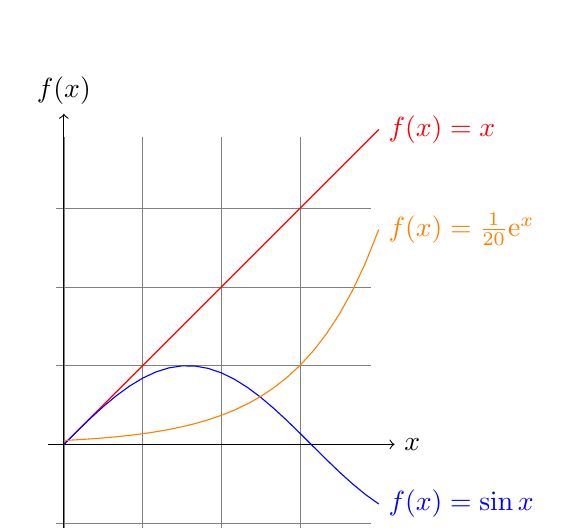
\begin{tikzpicture}[domain=0:4]
      \draw[very thin,color=gray] (-0.1,-1.1) grid (3.9,3.9);
      \draw[->] (-0.2,0) -- (4.2,0) node[right] {$x$};
      \draw[->] (0,-1.2) -- (0,4.2) node[above] {$f(x)$};
      \draw[color=red] plot (\x,\x) node[right] {$f(x) =x$};
      \draw[color=blue] plot (\x,{sin(\x r)}) node[right] {$f(x) = \sin x$};
      \draw[color=orange] plot (\x,{0.05*exp(\x)}) node[right] {$f(x) = \frac{1}{20} \mathrm e^x$};
      \end{tikzpicture}

\section{Conclusion}
This paper is to demonstrate that you have done well with {\TeX}pen.




\clearpage
%%%%%%%%%%%%%%%%%%%%%%%%%%%%%%%%%%%%%%%%%%%%%%
%%%%%%%%%%%%%%%%%%%%%%%%%%%%%%%%%%%%%%%%%%%%%%
%%%%%%%%%%%%%%%    Bib here                    %%%%%%%%%%%%%%%%%%
%%%%%%%%%%%%%%%%%%%%%%%%%%%%%%%%%%%%%%%%%%%%%%

%% The bib style options
%\bibliographystyle{apa}%{ieeetr}%{plain}
%% The bib file
%\bibliography{somefile.bib}

\end{document}
%%%%%%%%%%%%% END of DOCUMENT %%%%%%
%%%%%%%%%%%%%%%%%%%%%%%%%%%%%%%%%%%%%%%%%%%%%%
%%%%%%%%%%%%%%%%%%%%%%%%%%%%%%%%%%%%%%%%%%%%%%